\documentclass[epsfig,10pt,fullpage]{article}

\newcommand{\LabNum}{12}
\newcommand{\CommonDocsPath}{../../../common/docs}
\addtolength{\textwidth}{1.5in}
\addtolength{\oddsidemargin}{-0.75in}
\addtolength{\topmargin}{-0.75in}
\addtolength{\textheight}{1.5in}
\addtolength{\evensidemargin}{0.75in}
\setlength\parindent{0pt}
\raggedbottom

\usepackage{ae,aecompl}
\usepackage{epsfig,float,times}
\usepackage[hypcap]{caption}
\usepackage[pdftex, colorlinks]{hyperref}
\usepackage{graphicx}
\usepackage[usenames, dvipsnames]{color}
\usepackage{rotating}
\usepackage{tikz}
\usetikzlibrary{automata,positioning}
\usepackage{placeins}

\widowpenalty 10000
\clubpenalty 10000

\newcommand{\red}[1]{{\color{red}\sf{#1}}}
\newcommand{\green}[1]{{\color{green}\sf{#1}}}
\newcommand{\blue}[1]{{\color{blue}\sf{#1}}}
\definecolor{PineGreen}{rgb}{0.0, 0.47, 0.44}
\definecolor{ForestGreen}{rgb}{0.13, 0.55, 0.13}
\definecolor{Brown}{rgb}{0.59, 0.29, 0.0}

\newcommand{\UPDatePublished}{Oct 2021}
\newcommand{\versnum}{21.1} %version number quartus/AMP
\newcommand{\quartusname}{Quartus\textsuperscript{\textregistered} Prime}	
\newcommand{\UPTextBar}{For \quartusname{} \versnum{}}
\newcommand{\thisyear}{2021 } %for copyright
\newcommand{\company}{FPGAcademy.org}
\newcommand{\longteamname}{FPGAcademy.org}
\newcommand{\teamname}{FPGAcademy}
\newcommand{\website}{FPGAcademy.org}

\newcommand{\productAcronym}{AMP}
\newcommand{\productNameShort}{Monitor Program}

\newcommand{\productNameMedTM}{A Monitor Program}
\newcommand{\productNameMed}{A Monitor Program}

%\newcommand{\headerLogoFilePath}[1]{#1/FPGAcademy.png}

% listings is a package that supports encapsulating source code in LaTeX conveniently
\usepackage{listings}

\def\expandparam\lstinputlisting[#1]#2{\edef\tmp{\noexpand\lstinputlisting[#1]{#2}}\tmp}

%%%%%%%%%%%%%%%%%%%% Source Code Formatting %%%%%%%%%%%%%%%%%%%%
\definecolor{globalCommentColour}{rgb}{0.588,0.588,0.588}

%%%%%%%%%%%%%%%%%%%%%%%%%%%%%%%%%%%%%%%%%%%%%%%%%%%%
% Defining language style
% NiosII ASM
\lstdefinelanguage[NiosII]{Assembler} {
  morekeywords={add, addi, and, andhi, andi, beq, bge, bgeu, bgt, bgtu, ble,  bleu, blt, bltu, bne, br, break,
  bret, call, callr, cmpeq, cmpeqi, cmpge, cmpgei, cmpgeu, cmpgeui, cmpgt, cmpgti, cmpgtu, cmpgtui, cmple,
  cmplei, cmpleu, cmpleui, cmplt, cmplti, cmpltu, cmpltui, cmpne, cmpnei, custom, div, divu, eret, flushd,
  flushda, flushi, flushp, initd, initda, initi, jmp, jmpi, ldb, ldbio, ldbu, ldbuio, ldh, ldhio, ldhu, ldhuio,
  ldw, ldwio, mov, movhi, movi, movia, movui, mul, muli, mulxss, mulxsu, mulxuu, nextpc, nop, nor, or, orhi, ori,
  rdctl, rdprs, ret, rol, roli, ror, sll, slli, sra, srai, srl, srli, stb, stbio, sth, sthio, stw, stwio,
  sub, subi, sync, trap, wrctl, wrtcl, wrprs, xor, xori, xorhi, xori},
  morekeywords=[2]{.abort, .ABORT, .align, .app-file, .ascii, .asciz, .balign, .byte, .comm, .data, .def,
  .desc, .dim, .double, .eject, .else, .end, .endef, .endif, .equ, .equiv, .err, .extern, .file, .fill, .float,
  .global, .globl, .hword, .ident, .if, .include, .int, .irp, .irpc, .lcomm, .lflags, .line, .linkonce, .ln,
  .list, .long, .macro, .mri, .nolist, .octa, .org, .p2align, .psize, .quad, .rept, .sbttl, .scl, .section,
  .set, .short, .single, .size, .sleb128, .skip, .space, .stadb, .stabn, .stabs, .string, .symver, .tag,
  .text, .title, .type, .val, .uleb128, .word},
  morekeywords=[3]{et, bt, gp, sp, fp, ea, sstatus, ra, pc, status, estatus, bstatus, ienable, ipending, cpuid,
  exception, pteaddr, tlbacc, tlbmisc, eccinj, badaddr, config, mpubase, mpuacc},
  sensitive=t,
  alsoletter=.,
  morestring=[b]",
  morecomment=[s]{/*}{*/},
  morecomment=[l]\#,
}[keywords,comments,strings]
   
%% NOTE: morekeywords=[2] are GNU directives.
   
\definecolor{niosInstructionColour}{rgb}{0.000,0.608,0.000}
\definecolor{niosDirectiveColour}{rgb}{0.000,0.000,0.902}
\definecolor{niosSpecialRegColour}{rgb}{0.000,0.000,0.000}
\definecolor{niosStringColour}{rgb}{0.808,0.482,0.000}
   
%% NOTE: To make bold use: =\bfseries\color{<colour>}
\lstdefinestyle{defaultNiosStyle} {
  language=[NiosII]{Assembler},
  stringstyle=\color{niosStringColour},
  keywordstyle=\color{niosInstructionColour},
  keywordstyle=[2]\color{niosDirectiveColour},
  keywordstyle=[3]\itshape\color{niosSpecialRegColour}
}
%%%%%%%%%%%%%%%%%%%%%%%%%%%%%%%%%%%%%%%%%%%%%%%%%%%%

%%%%%%%%%%%%%%%%%%%%%%%%%%%%%%%%%%%%%%%%%%%%%%%%%%%%
% Defining language style
% ArmA9 ASM
\lstdefinelanguage[ArmA9]{Assembler} {
  morekeywords={ADC, ADD, ADDS, AND, ANDS, B, BAL, BEQ, BGE, BGT, BL, BLT, BIC, BKPT, BLX, BNE, BX, CDP, CLZ, CMN, CMP, EOR,
  EORS, LDC, LDM, LDR, LDRB, LDRBT, LDRH, LDRSB, LDRSH, LDRT, LSL, MCR, MLA, MOV, MOVW, MOVT, MRC, MRS, MSR, MUL, MVN, ORR, PLD,
  ROR, RSB, RSC, SBC, SMLAL, SMULL, STC, STM, STR, STRB, STRBT, STRH, STRT, SUB, SUBS, SWI, SWP, SWPB, TEQ, UMLAL,
  PUSH, POP, MOVS, RORS, LSR},
  morekeywords=[2]{.abort, .ABORT, .align, .app-file, .ascii, .asciz, .balign, .byte, .comm, .data, .def,
  .desc, .dim, .double, .eject, .else, .end, .endef, .endif, .equ, .equiv, .err, .extern, .file, .fill, .float,
  .global, .globl, .hword, .ident, .if, .include, .int, .irp, .irpc, .lcomm, .lflags, .line, .linkonce, .ln,
  .list, .long, .macro, .mri, .nolist, .octa, .org, .p2align, .psize, .quad, .rept, .sbttl, .scl, .section,
  .set, .short, .single, .size, .sleb128, .skip, .space, .stadb, .stabn, .stabs, .string, .symver, .tag,
  .text, .title, .type, .val, .vectors, .uleb128, .word},
  morekeywords=[3]{SP, PC, MIDR, CTR, TCMTR, TLBTR, MPIDR, ID_PFR0, ID_PFR1, ID_DFR0, ID_MMFR0, ID_MMFR1, ID_MMFR2,
  ID_MMFR3, ID_ISAR0, ID_ISAR1, ID_ISAR2, ID_ISAR3, ID_ISAR4, CCSIDR, CLIDR, AIDR, CSSELR, TTBR0, TTRB1, TTBR2, DACR,
  DFSR, IFSR, ADFSR, AIFSR, DFAAR, IFAR, ICIALLUIS, BPIALLIS, PAR, ICIALLU, ICIMVAU, BPIALL, DCIMVAC, DCISW, V2PCWPR,
  DCCVAC, DCCSW, DDIMVAC, DCISW, TLBALLIS, TLBIMVAIS, TLBIASIDIS, TLBIMVAAIS, TLBIALL, TLBIMVA, TLBIASID, TLBIMVAA,
  PMCR, PMCNTENSET, PMCNTENCLR, PMOVSR, PMSWINC, PMSELR, PMXEVTYPER, PMXEVCNTR, PMUSERENR, PMINTENSET, PMINTENCLR,
  PRRR, NRRR, PLEIDR, PLEASR, PLEFSR, PLEUAR, PLEPCR, VBAR, MVBAR, ISR, FCSEIDR, CONTEXTIDR, TPIDRURW, TPIDRURO, TPIDRPRW},
  sensitive=f,
  alsoletter=.,
  morestring=[b]",
  morecomment=[s]{/*}{*/},
  morecomment=[l]{//},
}[keywords,comments,strings]
   
%% NOTE: morekeywords=[2] are GNU directives.
   
\definecolor{armInstructionColour}{rgb}{0.000,0.608,0.000}
\definecolor{armDirectiveColour}{rgb}{0.000,0.000,0.902}
\definecolor{armSpecialRegColour}{rgb}{0.000,0.000,0.000}
\definecolor{armStringColour}{rgb}{0.808,0.482,0.000}
   
\lstdefinestyle{defaultArmStyle} {
  language=[ArmA9]{Assembler},
  stringstyle=\color{armStringColour},
  keywordstyle=\color{armInstructionColour},
  keywordstyle=[2]\color{armDirectiveColour},
  keywordstyle=[3]\itshape\color{armSpecialRegColour}
}
%%%%%%%%%%%%%%%%%%%%%%%%%%%%%%%%%%%%%%%%%%%%%%%%%%%%

%%%%%%%%%%%%%%%%%%%%%%%%%%%%%%%%%%%%%%%%%%%%%%%%%%%%
% Defining language style
% FPGAcademy ASM
\lstdefinelanguage{ASM}{
  morekeywords = [1]{mv, mvt, mvne, mvcc, add, sub, st, ld, and, b, bne, beq, bcc, bcs},
  morekeywords = [2]{word, define},
  keywordstyle = [1]\color{ForestGreen},
  keywordstyle = [2]\color{blue},
  sensitive = true,
  morecomment = [l]{//},
}

\lstset{
  language = ASM,
  basicstyle=\small\color{black}\ttfamily,
  commentstyle=\small\color{Brown}\itshape\ttfamily,
  showstringspaces=false,
  frame=none, %lines % boxed listings
  breaklines=true,
  breakatwhitespace=true,
  tabsize=3
}
%%%%%%%%%%%%%%%%%%%%%%%%%%%%%%%%%%%%%%%%%%%%%%%%%%%%

%%%%%%%%%%%%%%%%%%%%%%%%%%%%%%%%%%%%%%%%%%%%%%%%%%%%
% Defining language style
% Java
\definecolor{javaStringColour}{rgb}{0.808,0.482,0}
%%%%%%%%%%%%%%%%%%%%%%%%%%%%%%%%%%%%%%%%%%%%%%%%%%%%

%%%%%%%%%%%%%%%%%%%%%%%%%%%%%%%%%%%%%%%%%%%%%%%%%%%%
% Defining language style
% C
\definecolor{CStringColour}{rgb}{0.808,0.482,0}

\lstset{
  language = C,
  basicstyle=\small\color{black}\ttfamily, 
  commentstyle=\small\color{PineGreen}\itshape\ttfamily,
  keywordstyle=\small\color{blue}\bfseries\ttfamily,
  showstringspaces=false,
  frame=none, %lines % boxed listings
  breaklines=true,
  breakatwhitespace=true,
  tabsize=3
}
%%%%%%%%%%%%%%%%%%%%%%%%%%%%%%%%%%%%%%%%%%%%%%%%%%%%

%%%%%%%%%%%%%%%%%%%%%%%%%%%%%%%%%%%%%%%%%%%%%%%%%%%%
% Defining language style
% Verilog
\definecolor{verilogCommentColour}{rgb}{0.000,0.502,0.000}

\lstdefinestyle{defaultVerilogStyle} {
  language={Verilog},
  keywordstyle=\color{blue},
  commentstyle=\color{verilogCommentColour}
}
%%%%%%%%%%%%%%%%%%%%%%%%%%%%%%%%%%%%%%%%%%%%%%%%%%%%

%%%%%%%%%%%%%%%%%%%%%%%%%%%%%%%%%%%%%%%%%%%%%%%%%%%%
% Defining language style
% VHDL
\lstdefinestyle{defaultVHDLStyle} {
  language={VHDL},
  keywordstyle=\color{blue},
  commentstyle=\color{verilogCommentColour}
}
%%%%%%%%%%%%%%%%%%%%%%%%%%%%%%%%%%%%%%%%%%%%%%%%%%%%

%%%%%%%%%%%%%%%%%%%%%%%%%%%%%%%%%%%%%%%%%%%%%%%%%%%%
% Defining language style
% LaTeX
\lstdefinelanguage[LocalLaTeX]{TeX}[LaTeX]{TeX}{moretexcs={bf, it, sf, lstset},}

\lstdefinestyle{defaultLocalLatexStyle} {
  language=[LocalLatex]{TeX},
  keywordstyle=\color{blue}\bfseries,
  keywordstyle=[2]\color{blue},
  keywordstyle=[3]\color{blue}\bfseries
}
%%%%%%%%%%%%%%%%%%%%%%%%%%%%%%%%%%%%%%%%%%%%%%%%%%%%

%%%%%%%%%%%%%%%%%%%%%%%%%%%%%%%%%%%%%%%%%%%%%%%%%%%%
% Defining language style
% Default
\lstset{
  basicstyle=\small\color{black}\ttfamily,
  commentstyle=\small\color{globalCommentColour}\itshape\ttfamily,
  keywordstyle=\small\color{blue}\bfseries\ttfamily,
  showstringspaces=false,
  frame=none, %lines % boxed listings
  breaklines=true,
  breakatwhitespace=true,
  tabsize=3
}
%%%%%%%%%%%%%%%%%%%%%%%%%%%%%%%%%%%%%%%%%%%%%%%%%%%%


\hypersetup{
  pdftitle={Digital Logic Lab Exercise \LabNum},
  linkcolor=blue,
  hyperindex=true,
  pdfauthor={FPGAcademy.org},
  pdfkeywords={FPGAcademy.org, FPGAcademy, Lab, Exercise, Digital Logic},
  bookmarks,
  bookmarksopen=false,
  filecolor=blue,
  pdfstartview={FitH},
  urlcolor=blue,
  plainpages=false,
  pdfpagelabels=true,
  linkbordercolor={1 1 1} %no color for link border
}



\begin{document}

\centerline{\huge Digital Logic}
~\\
\centerline{\huge Laboratory Exercise \LabNum}
~\\
\centerline{\large Basic Digital Signal Processing}
~\\

This is an exercise in using the audio coder/decoder (CODEC) on the Intel\textsuperscript{\textregistered} DE1-SoC or DE2-115 board.  
The exercise involves connecting a microphone to the audio CODEC to provide input sound, 
altering the received sound by filtering out noise, and then playing the resulting 
sound through speakers/headphones. In addition to a DE-series board, a microphone and
speakers or headphones are required.


\section*{Background}
\addcontentsline{toc}{1}{Background}
Sounds, such as speech and music, are signals that change over time. The amplitude of a 
signal determines the volume at which we hear it. The way the signal changes over time 
determines the type of sounds we hear. For example, an 'ah' sound is represented by a waveform 
shown in Figure~\ref{fig:original_waveform}.

\begin{figure}[H]
\centering
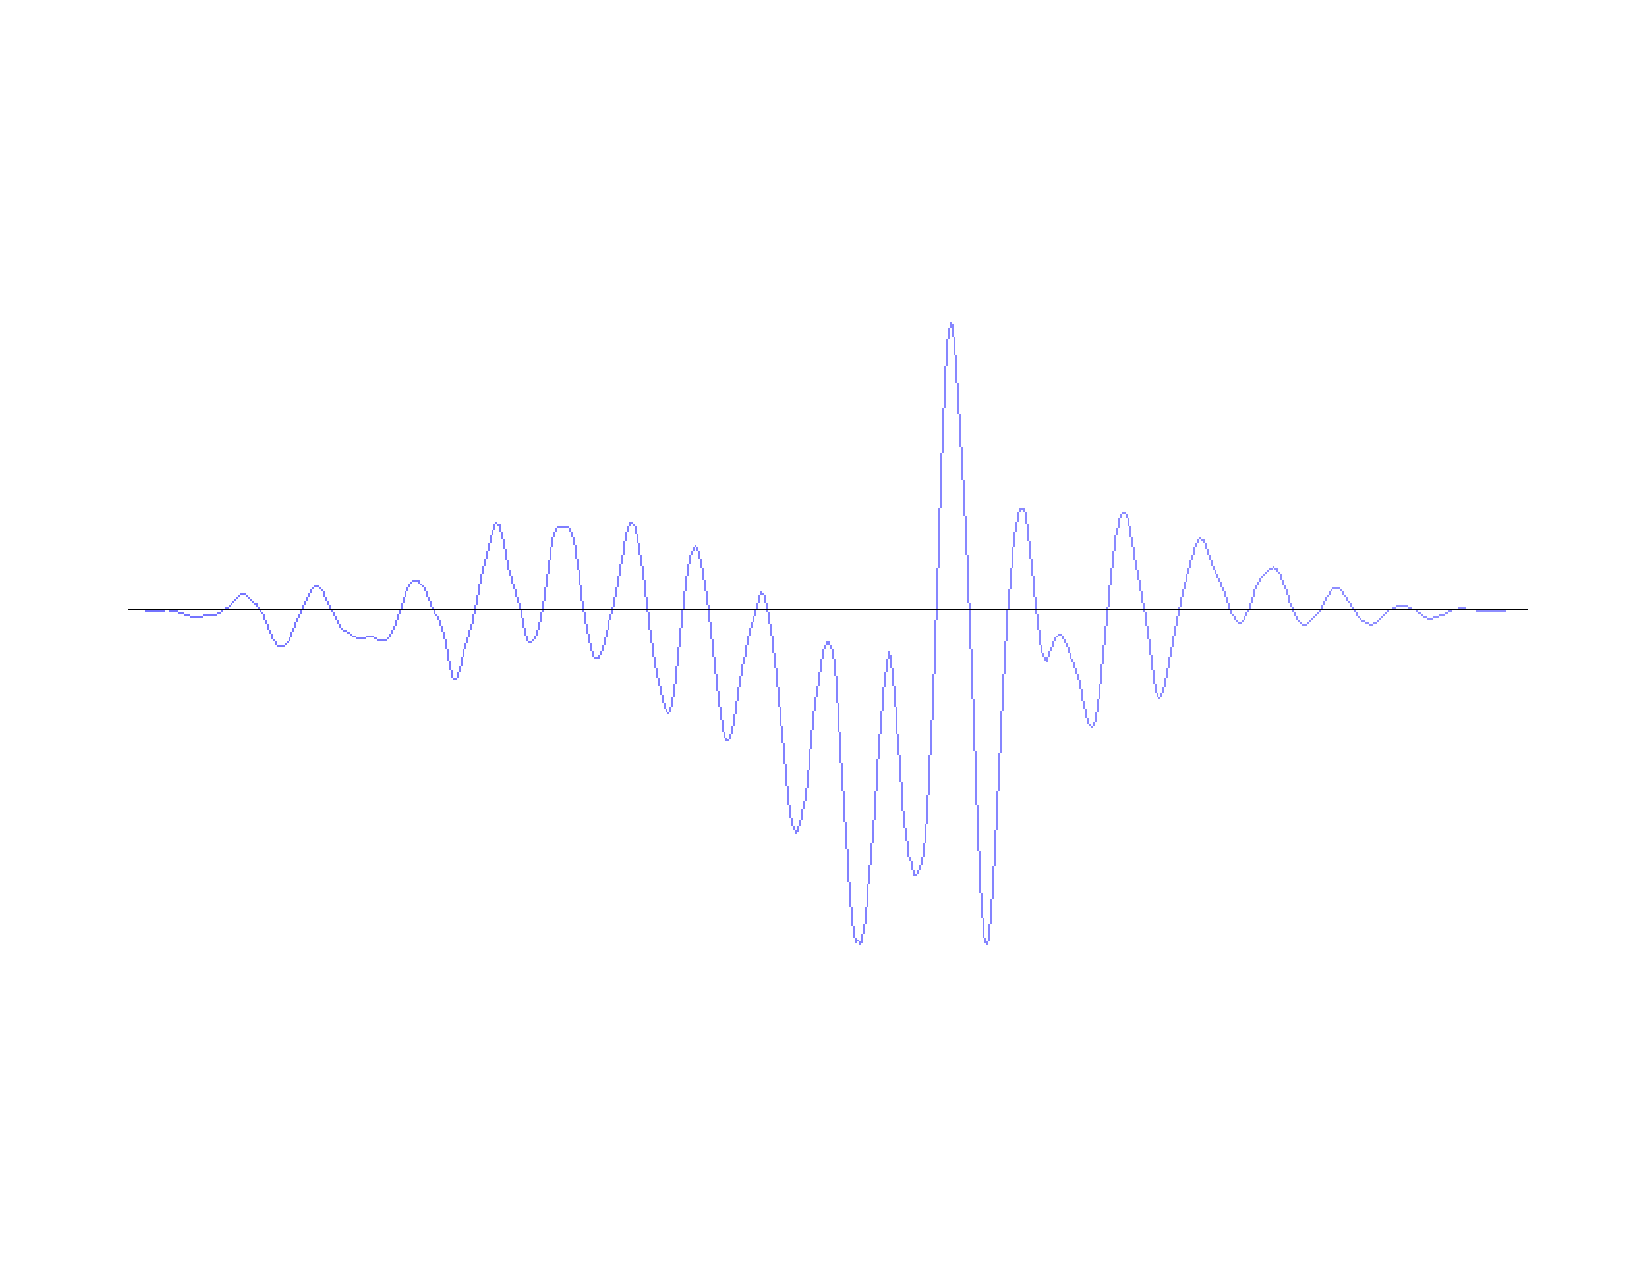
\includegraphics[width=4.5in]{figures/sound_wave_ah.pdf}
\caption{A waveform for an 'ah' sound.}
\label{fig:original_waveform}
\end{figure}

The waveform is an analog signal, which can be stored in a digital form by using a relatively 
small number of samples that represent the analog values at certain points in time. The process 
of producing such digital signals is called {\it sampling}.

\begin{figure}[H]
\centering
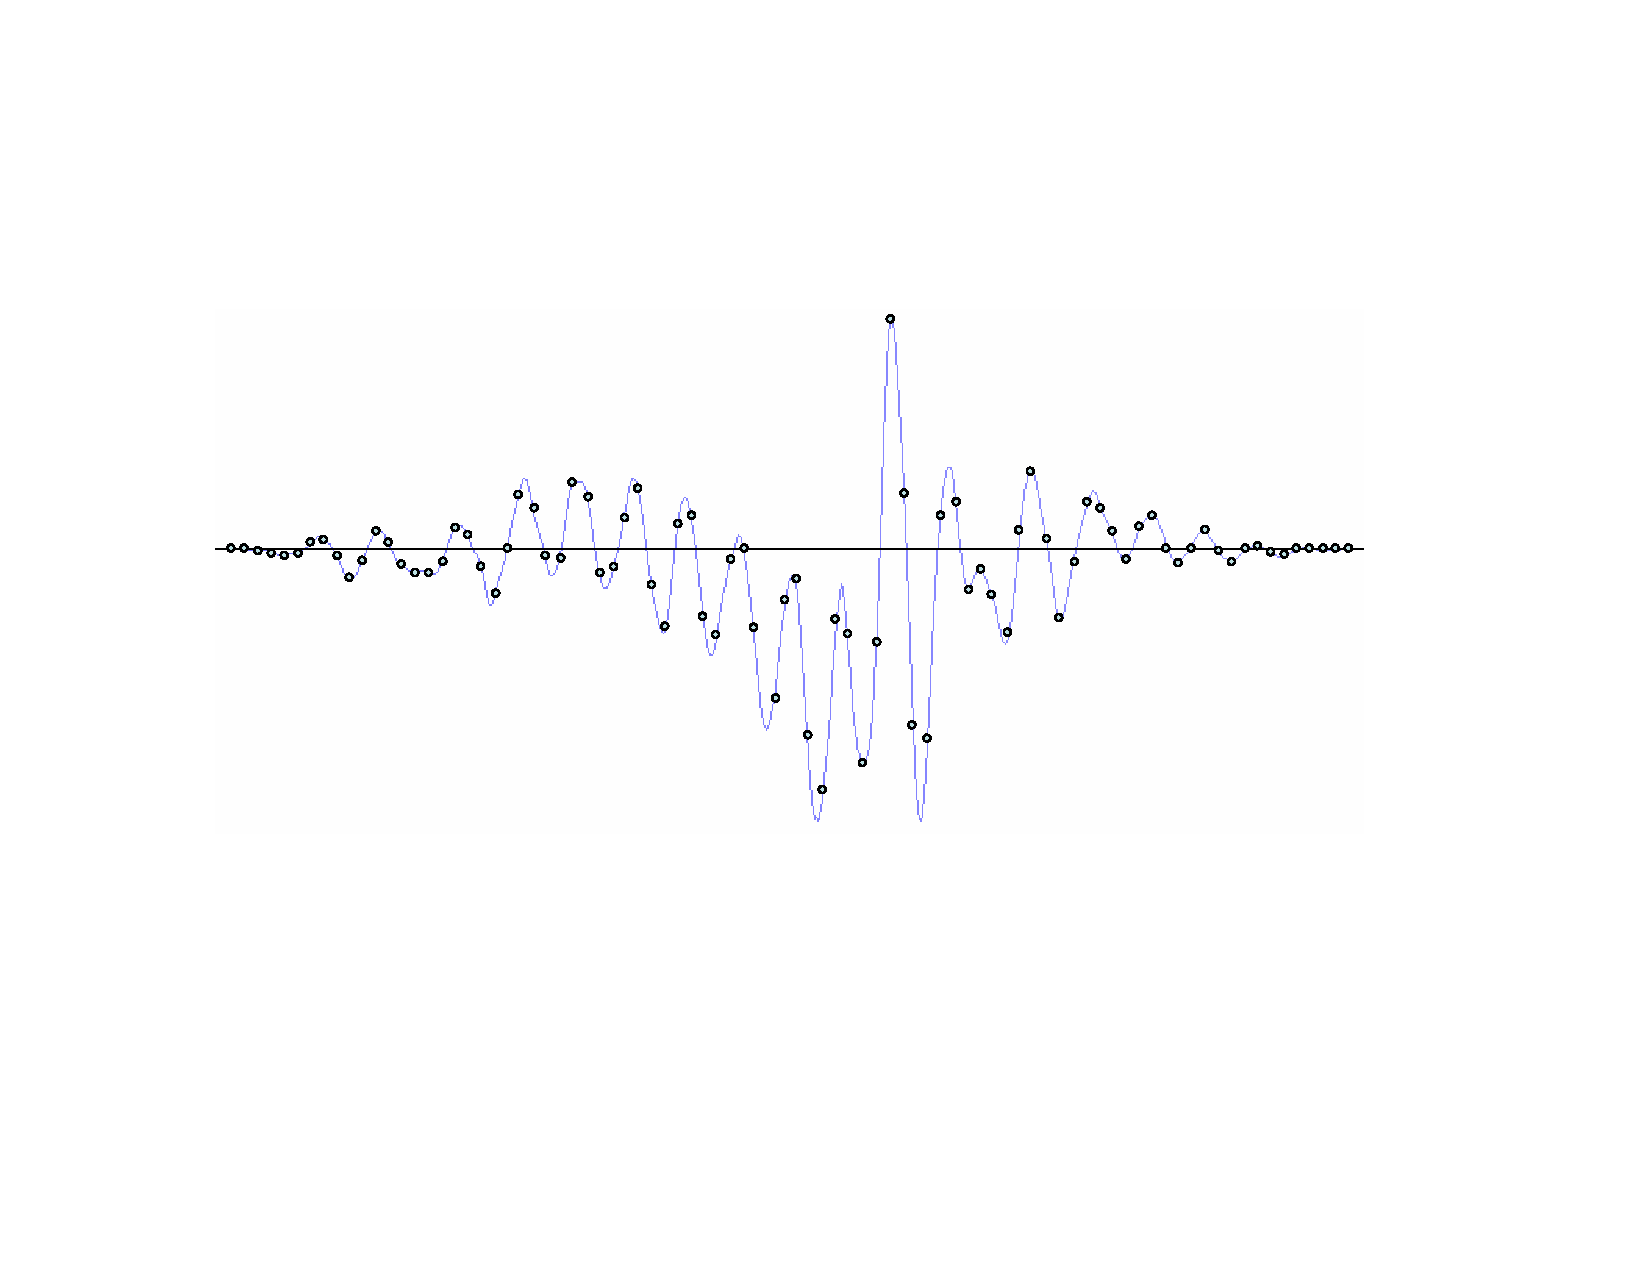
\includegraphics[width=4.5in]{figures/sampled_waveform.pdf}
\caption{A sampled waveform for an 'ah' sound.}
\label{fig:sampled_waveform}
\end{figure}

The points in Figure~\ref{fig:sampled_waveform} provide a sampled waveform. All points are spaced 
equally in time and they trace the original waveform.

~\\
The Intel DE1-SoC, and DE2-115 board are equipped with an audio CODEC capable of sampling sound from a microphone and providing it
as input to a circuit. By default, the CODEC provides 48000 samples per second, which is sufficient to accurately represent
audible sounds.

~\\
This exercise involves the design of several circuits that take input from a microphone
through the CODEC, record and process this sound data, and then play it back through 
speakers. To simplify the task, a simple system that can record and playback sounds on
your DE-series board is provided as a "starter kit". The system, shown in 
Figure~\ref{fig:audio_system}, comprises a {\sf Clock Generator}, an
{\sf Audio CODEC Interface}, and an {\sf Audio/Video Configuration} modules. This interface is 
a simplified version of the Intel
University Program Audio IP Core that is provided on Intel's FPGA University Program website.

\begin{figure}[H]
\centering
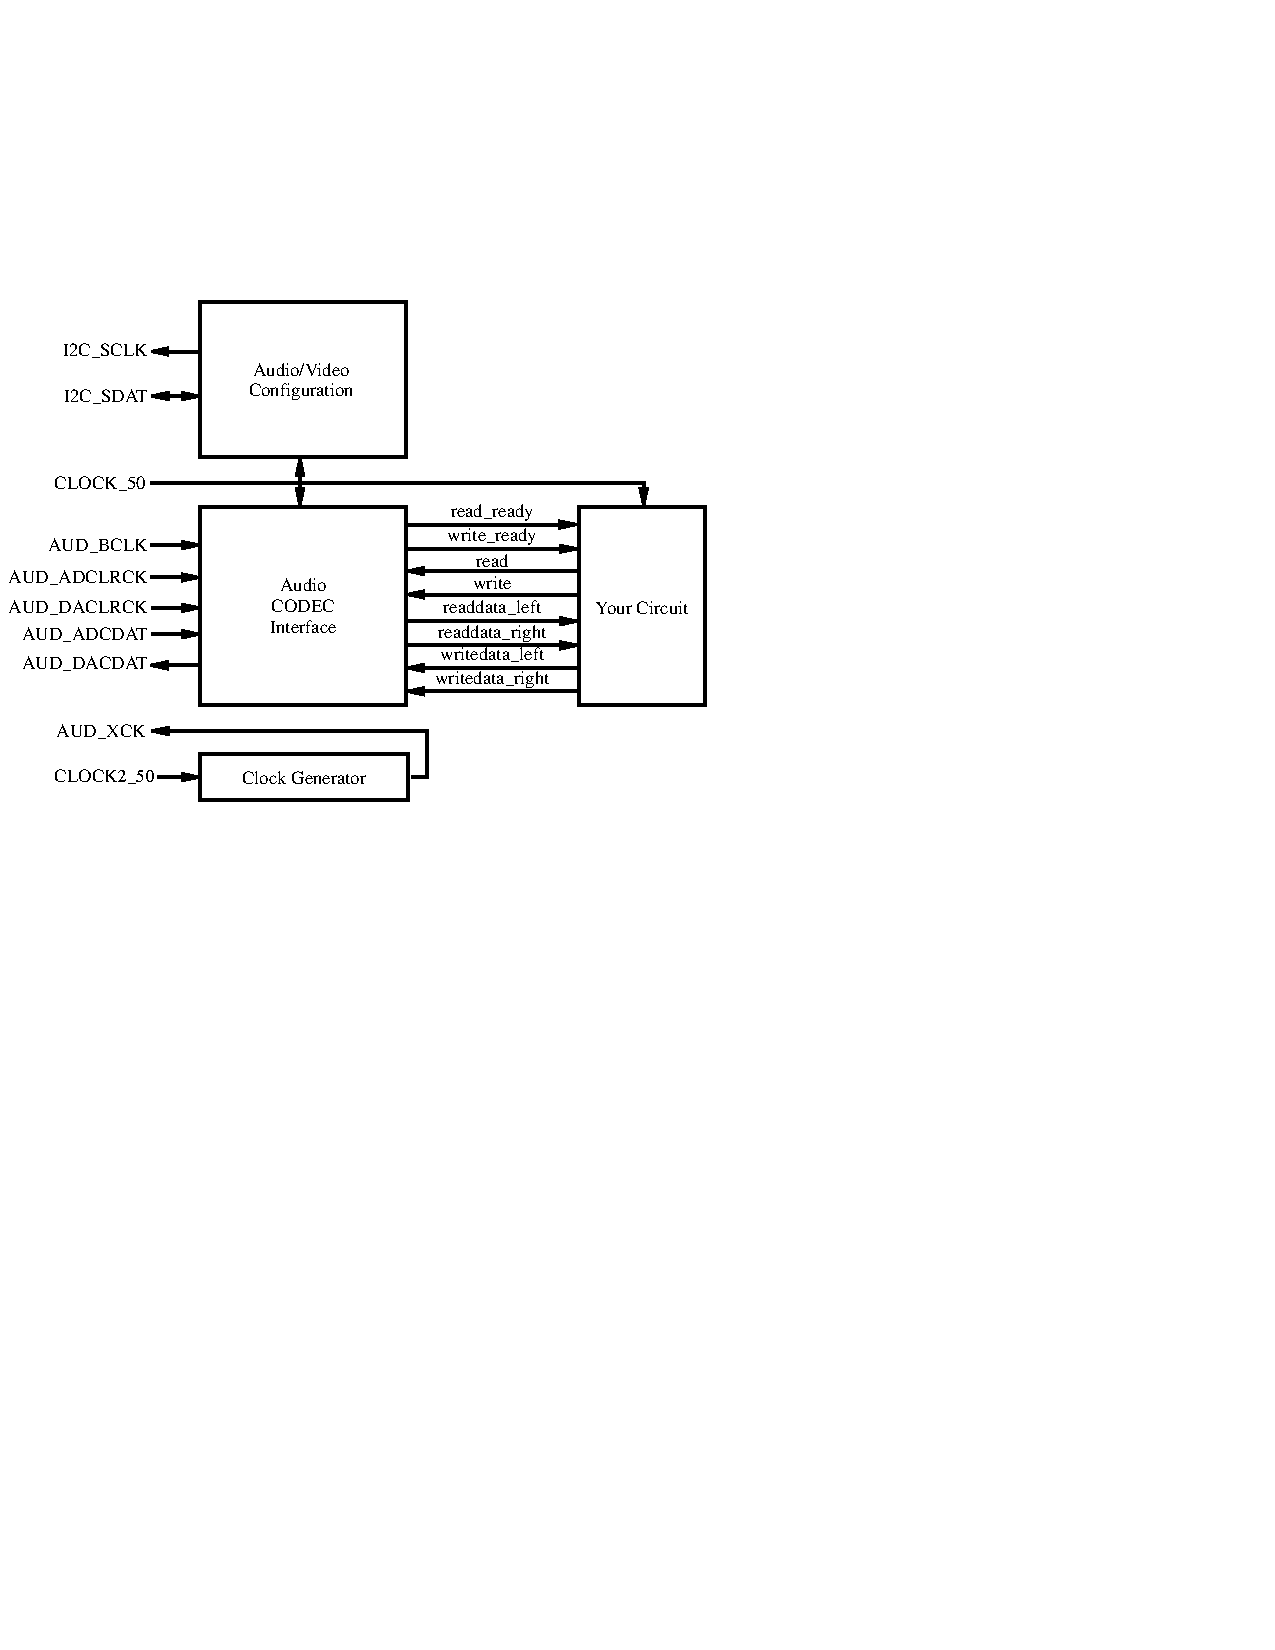
\includegraphics{figures/audio_system.pdf}
\caption{Audio System for this exercise.}
\label{fig:audio_system}
\end{figure}

The left-hand side of Figure~\ref{fig:audio_system} shows the inputs and outputs of the system. These I/O ports
supply the clock inputs, as well as connect the {\sf Audio CODEC} and {\sf Audio/Video Configuration} modules to the corresponding
peripheral devices on the Intel DE1-SoC and DE2-115 board. In the middle of the figure, a set 
of signals to and from the {\sf Audio CODEC Interface} module is shown. These signals 
allow the circuit depicted on the right-hand side to record sounds from a microphone and 
play them back via speakers.

~\\
The system works as follows. Upon reset, the {\sf Audio/Video Configuration} begins an autoinitialization sequence. The sequence sets up the
audio device to sample microphone input at a rate of 48kHz and produce output through 
the speakers at the same rate.
Once the autoinitialization is complete, the {\sf Audio CODEC} begins reading the data from the microphone once every 48000$^{th}$ of a second, and sends it
to the {\sf Audio CODEC Interface} core in the system. Once received, the sample is stored in a 128-element buffer in the {\sf Audio CODEC Interface} core.
The first element of the buffer is always visible on the {\sf readdata\_left} and {\sf readdata\_right} outputs when the {\sf read\_ready} signal is asserted.
The next element can be read by asserting the {\sf read} signal, which ejects the current sample and a new one appears one or more clock cycles later, if
the {\sf read\_ready} signal is asserted.

~\\
To output sound through the speakers a similar procedure is followed. Your circuit should observe the {\sf write\_ready} signal, and if asserted
write a sample to the Audio CODEC by providing it at the {\sf writedata\_left} and {\sf writedata\_right} inputs and asserting the {\sf write} signal.
This operation stores a sample in a buffer inside of the {\sf Audio CODEC Interface}, which will then send the sample to the speakers at the right time.

~\\
A starter kit that contains this design is provided as part of this exercise.

\section*{Part I}
\addcontentsline{toc}{2}{Part I}
In this part of the exercise, you are to make a simple modification to the provided
starter kit circuit to pass the input from the microphone to the speakers. You should
take care to read data from and write data to the {\sf Audio CODEC Interface} only when its ready signals are asserted.

~\\
Compile your circuit and download it onto an Intel DE1-SoC or DE2-115 board. Connect microphone and speakers to the {\sf Mic} and {\sf Line Out}
ports of the board and speak to the microphone to hear your voice through the speakers.

\section*{Part II}
\addcontentsline{toc}{3}{Part II}
In this part, you will learn a basic signal processing technique known as {\it filtering}. Filtering is a process of adjusting a signal -
for example, removing noise. Noise in a sound waveform is represented by small, but frequent changes to the amplitude of the signal. A simple logic
circuit that achieves the task of noise-filtering is an averaging Finite Impulse Response (FIR) filter. The schematic diagram of the filter
is shown in Figure~\ref{fig:eight_tap_fir_filter}.

\begin{figure}[H]
\centering
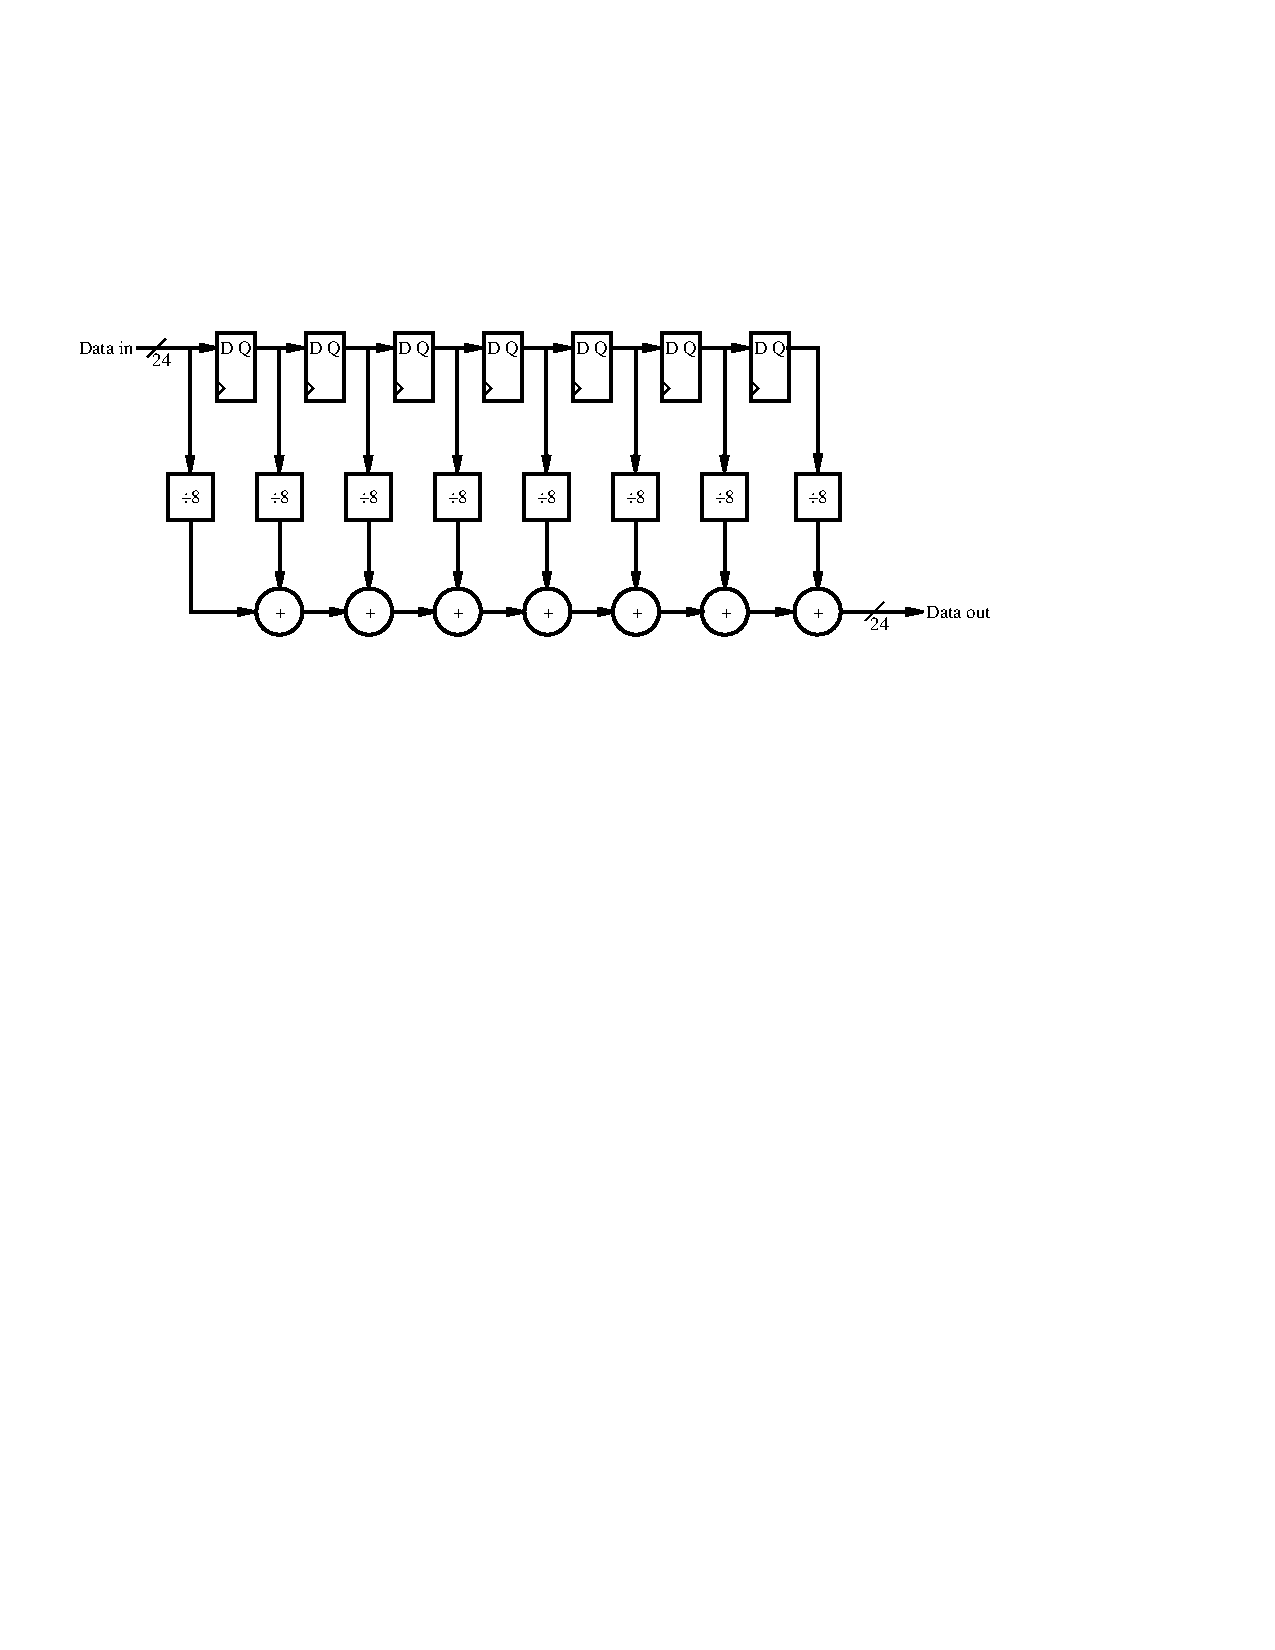
\includegraphics{figures/eight_tap_fir_filter.pdf}
\caption{A simple averaging FIR filter.}
\label{fig:eight_tap_fir_filter}
\end{figure}

An averaging filter, like the one shown in Figure~\ref{fig:eight_tap_fir_filter}, removes noise from a sound by averaging the values of
adjacent samples. In this particular case, it removes small deviations in sound by looking at changes in the adjacent 8 samples.
When using low-quality microphones, this filter should remove the noise produced when you speak to the microphone, making your voice sound clearer.

~\\
You are to implement the circuit shown in Figure~\ref{fig:eight_tap_fir_filter} to process the sound from the microphone, and output the filtered sound
through the speakers. Do you notice any difference between the quality of sound in this part as compared to Part I?

~\\
{\bf NOTE:}
~\\
It is possible to obtain high-quality microphones with noise-canceling capabilities. In such circumstances, you are unlikely
to hear any effect from using this filter. If this is the case, we suggest introducing some noise into the sound by adding
the output of the circuit in Figure~\ref{fig:noise_circuit} to the sample produced by the {\sf Audio CODEC}.

\begin{figure}[h]
\begin{center}
\begin{minipage}[t]{12.5 cm}
\begin{tabbing}
LIBRARY ieee;\\
USE ieee.std\_logic\_1164.all;\\
USE ieee.std\_logic\_signed.all;\\
~\\
ZZ\=PORT ~( \=Reset, Clock, RunZZ \=: BUFFERZZ\=STD\_LOGIC;\kill
ENTITY noise\_generator IS\\
\>PORT ( \>CLOCK\_50, read\_s \>:    IN \>STD\_LOGIC;\\
\>\>noise \>: OUT \>STD\_LOGIC\_VECTOR(23 DOWNTO 0));\\
END noise\_generator;\\
~\\
ZZ\=ZZ\=ZZ\=ZZ\=ZZ\=ZZ\=\kill
ARCHITECTURE Behavior OF upcount IS\\
\>SIGNAL counter : STD\_LOGIC\_VECTOR(2 DOWNTO 0);\\
\>SIGNAL Q : STD\_LOGIC\_VECTOR(9 DOWNTO 0);\\
~\\
BEGIN\\
\>PROCESS (Clock\_50)\\
\>BEGIN\\
\>\>IF (Clock'EVENT AND Clock = '1') THEN\\
\>\>\>IF (read\_s  = '1') THEN\\
\>\>\>\>counter $<$= counter + 1;\\
\>\>\>END IF;\\
\>\>END IF;\\
\>END PROCESS;\\
\>Q $<$= (OTHERS =$>$ counter(2));\\
\>noise $<$= Q\&counter\&"00000000000";\\
END Behavior;\\
~\rule{5.0in}{0in}
\end{tabbing}
\end{minipage}
\end{center}
\caption{Circuit to generate some noise.}
\label{fig:noise_circuit}
\end{figure}

The circuit is a simple counter, whose value should be interpreted as a signed value. The circuit should be clocked by a 50MHz clock, and the enable signal
should be driven high when the {\sf Audio CODEC} module can both produce and accept a new sample.

~\\
To hear the effect of the noise generator, add the values produced by the circuit to each sample of sound from the {\sf Audio CODEC} in the circuit in Part I.

\section*{Part III}
\addcontentsline{toc}{4}{Part III}
The implementation of the averaging filter in Part II may have been effective in removing some of the noise, and all of the noise produced by the noise generator.
However, if your microphone is of low-quality or you increase the width of the counter in the noise generator, the filter in Part II would be insufficient
to remove the noise. The reason for this is because the filter in Part II only looked at a very small time frame over which the sound waveform was
changing. This can be remedied by making the filter larger, taking an average of more samples.

~\\
In this part, you are to experiment with the size of the filter to determine the number of samples over which you have to average sound input to remove
background noise. To do this more effectively, use the design of an averaging FIR filter shown in Figure~\ref{fig:scalable_averaging_fir}.

\begin{figure}[H]
\centering
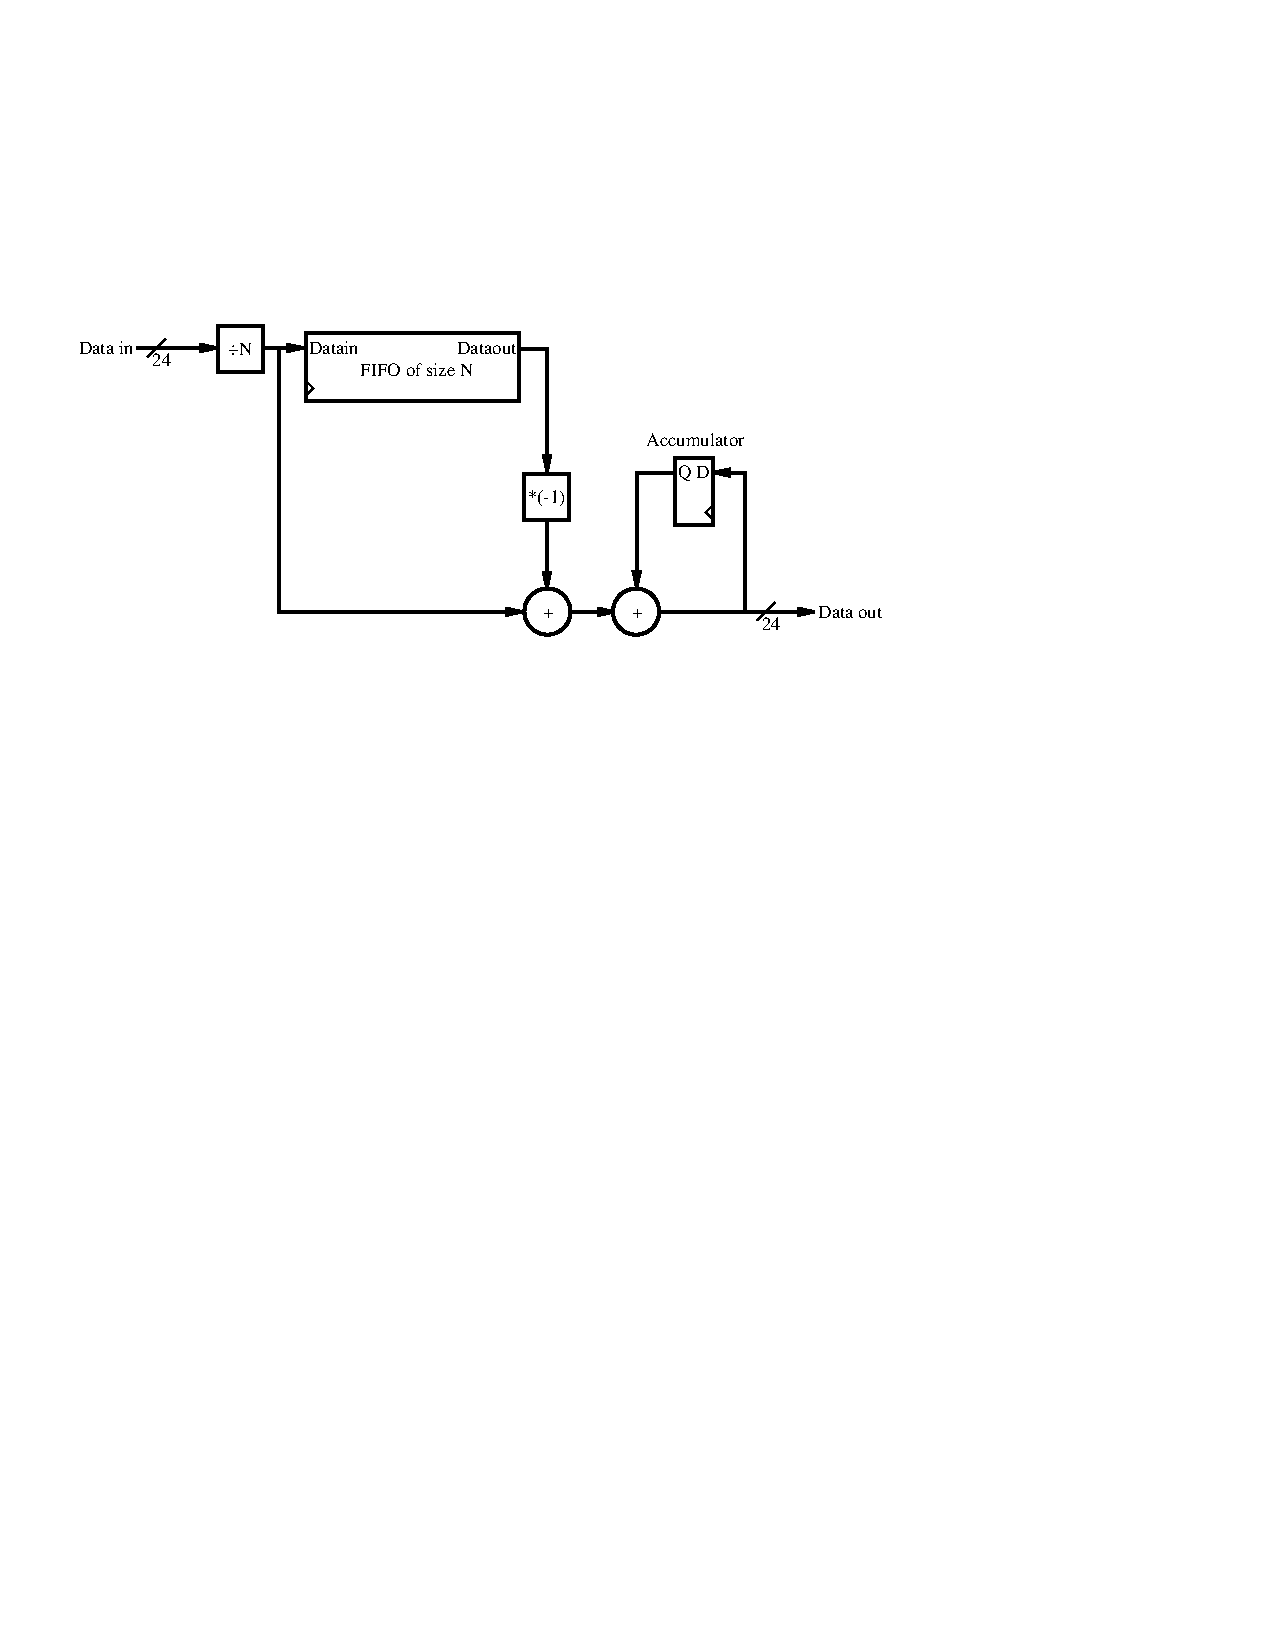
\includegraphics{figures/n_tap_averaging_fir_filter.pdf}
\caption{N-sample averaging FIR filter.}
\label{fig:scalable_averaging_fir}
\end{figure}

To compute the average of the last $N$ samples, this circuit first divides the input sample by $N$. Then, the resulting value
is stored it in a First-In First-out (FIFO) buffer of length $N$ and added to the accumulator. To make sure the value
in the accumulator is the average of the last $N$ samples, the circuit subtracts the value that comes out of the FIFO,
which represents the $(n+1)^{th}$ sample.

~\\
Implement, compile and download the circuit onto an Intel DE1-SoC, or DE2-115 board. Connect microphone and speakers to the {\sf Mic} and {\sf Line Out}
ports of the board and speak to the microphone to hear your voice through the speakers. Experiment with different values of $N$ to see what happens
to your voice and any background noise, remembering to divide the samples by appropriate value. We recommend experimenting with values of $N$ that are a power of 2, to make the division easier.

~\\
If you have a portable music player, with a connector such that you can supply input to your circuit through the {\sf Mic} port, try experimenting with
different sizes of the filter and its effect on the song you play. 


%%%%%%%%%%%%%%%%%%%%%%%%%%%%%%%%%%%%%%%%
%%% FPGAcademy Copyright Information %%%
%%%%%%%%%%%%%%%%%%%%%%%%%%%%%%%%%%%%%%%%

%Always put the copyright on a new page (clear page), with some vertical space from top
\clearpage
\vspace{1in}

\noindent

Copyright {\copyright} FPGAcademy.org. All rights reserved. FPGAcademy and the 
FPGAcademy logo are trademarks of FPGAcademy.org.  This document is provided 
"as is", without warranty of any kind, express or implied, including but not 
limited to the warranties of merchantability, fitness for a particular purpose 
and noninfringement. In no event shall the authors or copyright holders be 
liable for any claim, damages or other liability, whether in an action of 
contract, tort or otherwise, arising from, out of or in connection with the 
document or the use or other dealings in the document.
~\\
~\\
**Other names and brands may be claimed as the property of others.


\end{document}
